\documentclass[simplex.tex]{subfiles}
% NO NEED TO INPUT PREAMBLES HERE
% packages are inherited; you can compile this on its own

\onlyinsubfile{
\title{NeuroData SIMPLEX Report: Subfile}
}

\begin{document}
\onlyinsubfile{
\maketitle
\thispagestyle{empty}

The following report documents the progress made by the labs of Randal~Burns and Joshua~T.~Vogelstein at Johns Hopkins University towards goals set by the DARPA SIMPLEX grant.

%%%% Table of Contents
\tableofcontents

%%%% Publications
\bibliographystyle{IEEEtran}
\begin{spacing}{0.5}
\section*{Publications, Presentations, and Talks}
%\vspace{-20pt}
\nocite{*}
{\footnotesize	\bibliography{simplex}}
\end{spacing}
%%%% End Publications
}

\subsection{Multiscale Generalized Correlation (MGC)}

We developed the Multiscale Generalized Correlation method to better detect associations between two datasets $X$ and $Y$. We demonstrate that Oracle MGC is a consistent test statistic (power converge to 1 as sample size increases) under standard regularity conditions, is equivalently to the global correlation under linear dependency (i.e., each observation $X_i$ is a linear transformation of $Y_i$), and can be strictly better than the global correlation under common nonlinear dependencies. Thus Oracle MGC dominates the global correlation, and the sample MGC (i.e., choose the optimal scale by p-value map approximation, as the testing power are not available in the absence of the true model and training data) also empirically dominates the global correlation. A flowchart to illustrate the advantage of MGC is shown in Figure~\ref{fig:all}.  

\begin{figure}[h!]
\begin{cframed}
		\centering
		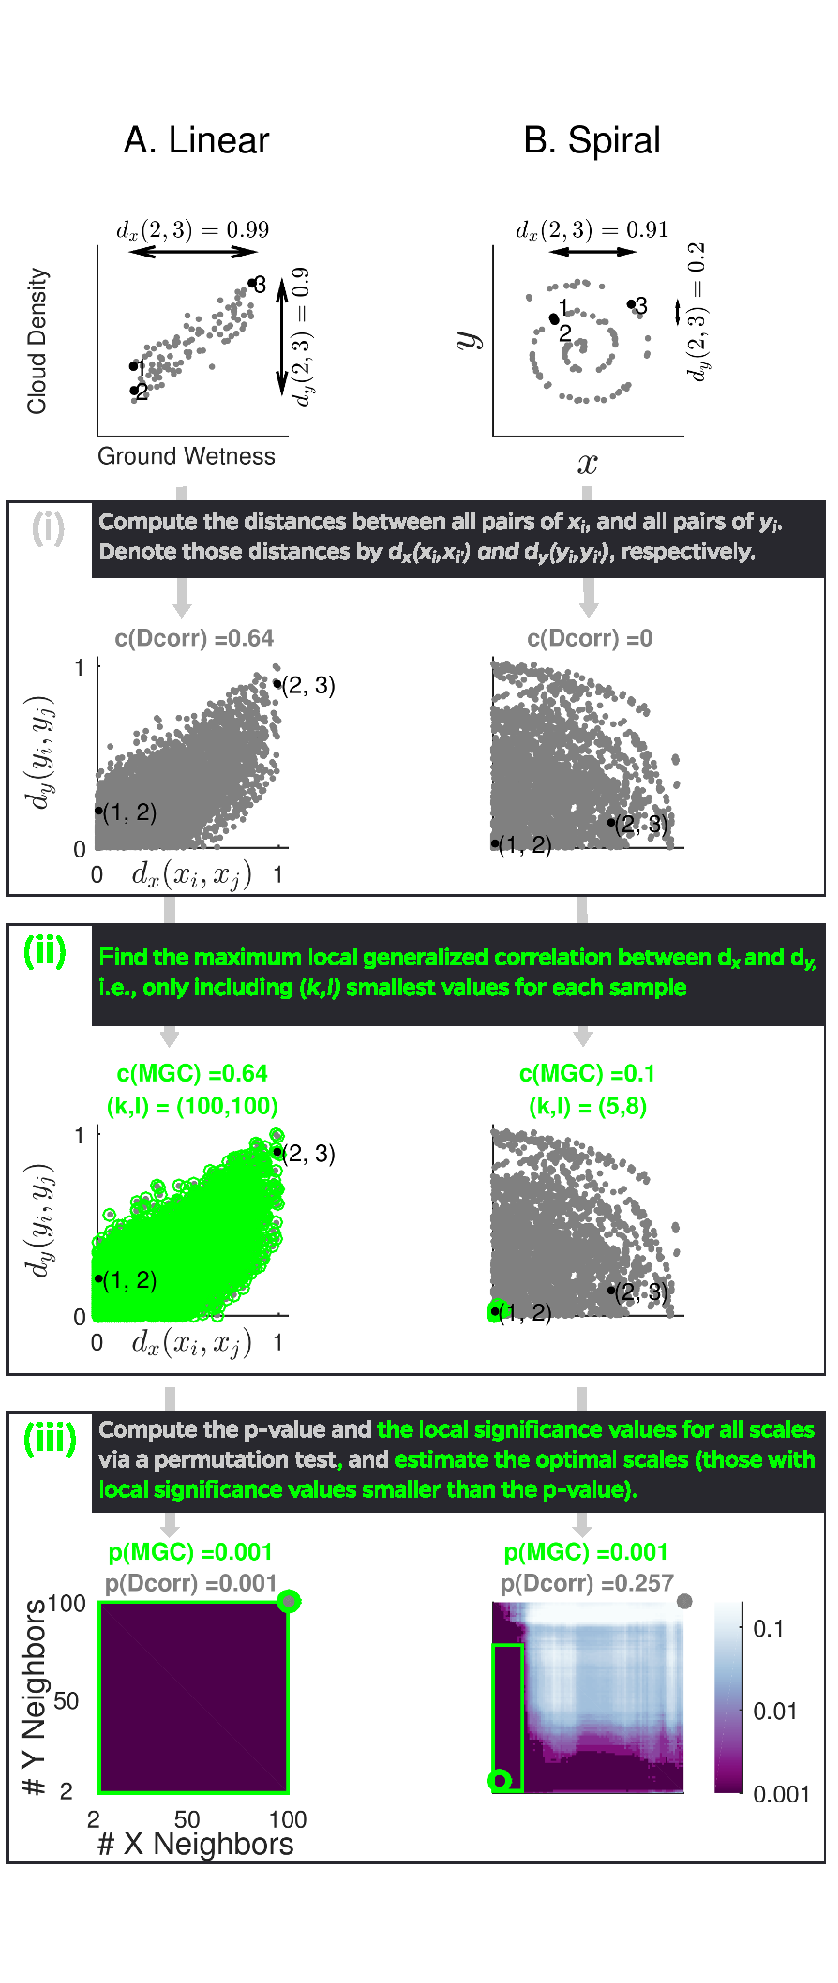
\includegraphics[width=0.6\textwidth]{../../figs/Fig1Allb}
		\label{fig:all}
		\end{cframed}
\end{figure}

The current draft is already uploaded to Arxiv, and will be submitted this month. As the next step, we are investigating the required sample size for MGC to achieve perfect power, as an effort to better understand its mechanism and better apply the methodology to real data testing. 

\end{document}
